\documentclass[11pt]{article}

%{{{ Packages
\usepackage[margin=1in]{geometry}
\usepackage{enumitem}
\usepackage{amsfonts}
\usepackage{amssymb}
\usepackage{amsmath}
\usepackage{centernot}
\usepackage{amsthm}
\usepackage{mathdots}
\usepackage{mathtools}
\usepackage[dvipsnames]{xcolor}
\usepackage[framemethod=TikZ]{mdframed}
\usepackage{microtype}
\usepackage{witharrows}
\setlength{\parindent}{0pt}
%}}}
%{{{ Custom commands
% Nice maths commands
\newcommand{\defeq}{:=}
\newcommand{\eqdef}{=:}
\newcommand{\abs}[1]{|#1|}
\newcommand{\norm}[1]{||#1||}
%\renewcommand{\dots}{...}
\newcommand{\msrspc}{\ensuremath{(X,\mathcal{B},\mu)}}
\newcommand{\homrel}{\stackrel{\partial}{\simeq}}
\newcommand{\homrelset}[1]{\stackrel{#1}{\simeq}}
\newcommand\restr[2]{{% we make the whole thing an ordinary symbol
  \left.\kern-\nulldelimiterspace % automatically resize the bar with \right
  #1 % the function
  \vphantom{\big|} % pretend it's a little taller at normal size
  \right|_{#2} % this is the delimiter
  }}
\newcommand{\relmiddle}[1]{\mathrel{}\middle#1\mathrel{}}
\newcommand{\rmv}{\relmiddle|}

% Custom operators
\makeatletter
\DeclareRobustCommand\bigop[1]{%
  \mathop{\vphantom{\sum}\mathpalette\bigop@{#1}}\slimits@
}
\newcommand{\bigop@}[2]{%
  \vcenter{%
    \sbox\z@{$#1\sum$}%
    \hbox{\resizebox{\ifx#1\displaystyle.9\fi\dimexpr\ht\z@+\dp\z@}{!}{$\m@th#2$}}%
  }%
}
\makeatother
\newcommand{\bigast}{\DOTSB\bigop{\ast}}

% Spaces
\newcommand{\ktor}{\mathbb{T}^k}
\newcommand{\R}{\mathbb{R}}
\newcommand{\C}{\mathbb{C}}
\newcommand{\Z}{\mathbb{Z}}
\newcommand{\N}{\mathbb{N}}

% Derivatives
\newcommand*{\pd}[3][]{\ensuremath{\frac{\partial^{#1} {#2}}{\partial {#3}^{#1}}}}
\newcommand{\grad}{\bigtriangledown}

% Vectors
\newcommand{\mv}[1]{\textbf{#1}}

%}}}
%{{{ Enviornments
% Definitions environment
\newenvironment{defin}
	{\begin{mdframed}[backgroundcolor=white, roundcorner=5pt, linewidth=1pt]}
	{\end{mdframed}}
\newcommand{\mdf}[1]{{\color{red} #1}}

% Important notes environment
\newenvironment{note}
	{\begin{mdframed}[backgroundcolor=white, linecolor=red, roundcorner=5pt, linewidth=1pt]\bfseries{Note:}\normalfont}
	{\end{mdframed}}

% Examples enviornmnet
\definecolor{mylg}{rgb}{0.9,0.9,0.9}
\newenvironment{eg}
	{\begin{mdframed}[backgroundcolor=myld,roundcorner=5pt,linewidth=0pt]\bfseries{Example:}}
	{\end{mdframed}}

% Theorem enviornment
\newtheorem{theorem}{Theorem}[section]
\newtheorem{prop}[theorem]{Proposition}
\newtheorem{cor}[theorem]{Corollary}
\newtheorem{lemma}[theorem]{Lemma}
%}}}
%{{{ Document metadata
\title{Intro to Topology - Overview}
\author{}
\date{}
%}}}

\begin{document}
\maketitle
\section{Key Definitions}
\begin{defin}
\begin{itemize}
	 \item Given maps $f,g:X\times I \to Y$, a \mdf{homotopy} from $f$ to $g$ is a continuous map  $F:X\times I \to Y$ such that $f_0=f$ and $f_1=g$.
		 If such a map exists we write $f\simeq g$.
	 \item Given paths $f,g:I \to X$. We say \mdf{$f$ is homotopic to $g$ relative to $\left\{x, y\right\}$} and write $f\homrel g$ if
		 \begin{enumerate}[label=(\roman*)]
			 \item $f(0)=g(0)=x$
			 \item $f(1)=g(1)=y$
			 \item There is a homotopy $F:I\times I \to X$ such that $f_0=f$, $f_1=g$ and for all $t\in I$, $f_t(0)=x$ and $f_t(1)=y$.
		 \end{enumerate}
	 \item A \mdf{pair} of spaces $(X,A)$ is a topological space together with a subspace $A\subseteq X$ using the subspace topology.
\end{itemize}
Assume we have a pair $(X,A)$.
\begin{itemize}
	 \item $A$ is a \mdf{retract} if there is a continuous map $r:X\to A$ such that $\restr{r}{A}=id_A$.
	 \item $X$ \mdf{deformation retracts} to $A$ if there exists a homotopy $F:X\times I \to X$ such that $f_0=id_X$, $f_1(X)=A$ and $\restr{f_t}{A}=id_A$ for all $t\in I$.
\end{itemize}
Assume we have topological space $X$ and $Y$ then,
\begin{itemize}
	\item $X$ is \mdf{homotopy equivalent} to $Y$ there exist maps $f:X\to Y$ and $g:Y\to X$ such that
	\[
g\circ f \simeq id_X \quad , \quad f\circ g \simeq id_Y
	\]
\item $X$ is \mdf{contractible} if it is homotopy equivalent to $\left\{pt\right\}$.
	
\end{itemize}
\end{defin}
\begin{note}
	\begin{align*}
		X \text{ deformation retracts to } A &\implies X \text{ contractible }\\
											 &\centernot\Longleftarrow
	\end{align*}
	The reverse does not hold because the contraction does not necessarily restrict to $id_A$.
\end{note}
\section{Fundamental Group}
\begin{defin}
	Given a pointed space $(X,x_0)$, a \mdf{loop} is a path $f:I \to X$ such that $f(0)=f(1)=x_0$.	

	We can then define an equivalence class for every loop $f$:
	\[
		[f]\defeq\left\{g \rmv g(0)=g(1)=x_0,\quad f\homrel g \right\}
	\]
	
	We then get the \mdf{fundamental group} defined to be
	\[
		\pi_1(X,x_0)\defeq\left\{[f] \rmv f \text{ a loop based at } x_0 \right\}
	\]

	This forms a group with the operation $[f]\cdot [g]=[f\ast g]$ and the identity element being the constant loop.
\end{defin}

\begin{theorem}
If $X$ is path connected and $x_0,x_1\in X$ then
\[
	\pi_1(X,x_0)=\pi_1(X,x_1)
\]
\end{theorem}

\begin{proof}
There exists a path $h:I\to X$ from $x_0$ to $x_1$.
Define $\overline{h}(s)\defeq h(1-s)$.
We can then define a base point change homomorphism which we claim is in fact an isomorphism.
\[
	\beta_h:\pi_1(X,x_0)\to\pi_1(X,x_1), \quad [f]\mapsto [\overline{h}\ast f \ast h]
\]
We can see this is in fact an isomorphism because $\beta_{\overline{h}}$ is a left and right inverse.
\end{proof}

\begin{defin}
	A map $p:\widetilde{X}\to X$ is a \mdf{covering map} if there is an open cover $\left\{U_\alpha\right\}$ of $X$ such that
	\[
		p^{-1}(U_\alpha)=\bigsqcup_\beta V_\alpha^\beta
	\]
	with each $V_\alpha^\beta$ open and such that $\restr{p}{V_\alpha^\beta}:V_\alpha^\beta\to U_\alpha$ is a homomorphism.

	The covering map is called \mdf{$n$-fold} if each $p^{-1}(x_0$ has $n$ elements for every $x_0$.

	Let $p:Y\to X$ and $q:Z\to X$ be coverings. These called \mdf{isomorphic} if there is a homeomorphism $h:Y\to Z$ such that
	\[
		q \circ h = p
	\]

	Let $p:\widetilde{X}\to X$ be a cover then a \mdf{deck transformation} is an isomorphism $\tau:\widetilde{X}\to\widetilde{X}$ such that $p\circ\tau=p$.

	\[
		\text{Deck}(p)\defeq\left\{\tau:\widetilde{X}\to\widetilde{X}\rmv\tau\text{ is a deck transformation }\right\}
	\]

	Given a covering $p:\widetilde{X}\to X$ and a map $f:Y\to X$, a \mdf{lift} of $f$ is a map $\widetilde{f}:Y\to\widetilde{X}$ such that $f=p\circ\widetilde{f}$.
\end{defin}

\begin{figure}[ht]
	\centering
	\includegraphics[width=4in]{basicdefs_diagrams.png}	
	\caption{Commutative diagrams defining various concepts}
\end{figure}

Here are some useful properties of lifts: 
\begin{enumerate}[label=(\roman*)]
	\item $\widetilde{f}:Y\to\widetilde{X}$ then $\widetilde{f}$ is a lift of $p\circ\widetilde{f}$.
	\item $\widetilde{f},\widetilde{g}:Y\to\widetilde{X}$ and $f\simeq g$ $\implies p\circ \widetilde{f}\simeq p\circ \widetilde{g}$ (homotopies descends).
	\item $\alpha, \beta: I \to \widetilde{X}$ such that $\alpha(1)=\beta(0)$ then $p\circ (\alpha\ast\beta)=(p\circ\alpha)\ast(p\circ\beta)$ (concatenation descends).
\end{enumerate}

\section{Homotopy Lifting Property}
\begin{defin}
	A map $p:Z\to X$ has the \mdf{homotopy lifting property} if given any homotopy $F:Y\times I \to X$ and any lift $g:Y\times\left\{0\right\}\to Z$ there exists a unique homotopy $\widetilde{F}Y\times I \to Z$ satisfying
	\begin{enumerate}[label=(\roman*)]
		\item $\widetilde{f}_0=g$
		\item $p\circ\widetilde{F}=F$
	\end{enumerate}
	i.e. given a homotopy and a lift of one endpoint, there exists a unique lift of that homotopy.

	As a special case where $Y=\left\{pt\right\}$, a map $p:Z\to X$ has the \mdf{path lifting property} if for any path $f:I\to X$, $x_0\in X$ and $\widetilde{x}_0\in p^{-1}(x_0)$ there exists a unique path $\widetilde{f}:I\to Z$ such that 
	\begin{enumerate}[label=(\roman*)]
		\item $\widetilde{f}(0)=\widetilde{x}_0$
		\item $p\circ\widetilde{f}=f$
	\end{enumerate}
\end{defin}

\begin{lemma}[Local Homotopy Lifting Property]
Let $p:\widetilde{X}\to X$ be a covering map and $F:Y\times I \to X$ a homotopy.
Suppose we have $g:Y\times\left\{0\right\}\to \widetilde{X}$.
Then for every $y\in Y$
\begin{enumerate}[label=(\alph*)]
	\item There exists an open neighbourhood $N\subseteq Y$ and a unique homotopy $\widetilde{F}_N:N\times I \to \widetilde{X}$ such that
		\begin{enumerate}[label=(\roman*)]
			\item $(\widetilde{f}_N)_0=g$.
			\item $p\circ\widetilde{F}_N=\restr{F}{N\times I}$.
		\end{enumerate}
	\item If $M\subseteq Y$ with $y\in M$ is another open neighbourhood for which \textit{(a)} holds then \textit{(a)} also holds for $M\cap N$ and
		\[
			\restr{\widetilde{F}_N}{(M\cap N)\times I)}=\restr{\widetilde{F}_M}{(M\cap N)\times I}=\widetilde{F}_{M\cap N}
		\]
\end{enumerate}
\end{lemma}
\begin{proof}
This has a very long proof.
\end{proof}

\begin{prop}
Covering maps $p:\widetilde{X}\to X$ have the homotopy lifting property.
\end{prop}

\begin{proof}
Let $P;\widetilde{X}\to X$ be a covering map.
Let $F:Y\times I \to I$ be a homotopy and choose soma arbitrary starting $g:Y\times\left\{0\right\}\to\widetilde{X}$.

We can cover $Y=\cup_\alpha N_\alpha$ such that \textit{(a)} and \textit{(b)} hold from the lemma.

We can then define a new homotopy by stitching these together:
\[
	\widetilde{F}:Y\times I \to \widetilde{X},\quad\quad \widetilde{F}(y, t)\defeq \widetilde{F}_{N_\alpha}(y, t)\;\;\text{if}\;\; y\in N_\alpha
\]
We do not get any ambiguity here thanks to property \textit{(b)} from the lemma.
The continuity of this construction follows from the pasting lemma.
\end{proof}

\begin{theorem}
Let $\omega_N:I\to S^1$ be defined by $\omega_n(s)=e^{2\pi i n s}$. Then
\[
	\pi_1(S^1,1)=\left\{[\omega_n] \rmv n\in\Z\right\}
\]
\end{theorem}

\begin{proof}
Define $\Phi:\Z\to\pi_1(S^1,1)$ by $n\mapsto [\omega_n]$. We claim this is an isomorphism.
For this define the following useful maps
\begin{align*}
	p(t)&=e^{2\pi i t}	\\
	\omega_n(t) &= e^{2\pi i n t} \\
	\widetilde{\omega}_n(t) &= nt \\
	\tau_m(t)&=t+m
\end{align*}
\begin{itemize}
	\item \underline{$\Phi$ is a group homomorphism.}

		Then we can see that indeed $\widetilde{\omega_n}:\R\to\R$ is a lift of $\omega_n$.
		One can also see through the linear homotopy that
		\[
			\widetilde{\omega}_{m+n}\homrel \widetilde{\omega}_m\ast(\tau_m\circ \widetilde{\omega}_n)
		\]
		Now given any $m, n\in\Z$ we have
		\[
		\begin{WithArrows}
			\Phi(m+n) &= [\omega_{n+m}] \Arrow{\text{lift}}\\
					  &= [p\circ\widetilde{\omega}_{n+m}] \Arrow{\text{homotopies descend}}\\
					  &= \left[p \circ \left(\widetilde{\omega}_m\ast\left(\tau_m\circ\widetilde{\omega}_n\right)\right)\right] \\
					  &= [p\circ\widetilde{\omega_m}]\cdot[p\circ\tau_m\circ\widetilde{\omega}_n] \Arrow{\text{deck transformation}}\\
					  &= [p\circ\widetilde{\omega_m}]\cdot[p\circ\widetilde{\omega}_n]\Arrow{\text{lift}}\\
					  &= [\omega_m]\cdot[\omega_n]\\
					  &= \Phi(m)\cdot\Phi(n)
		\end{WithArrows}
		\]
	\item \underline{$\Phi$ is surjective.}

		Choose any $[\alpha]\in\pi_1(S^1,1)$, we aim to find $n\in\N$ such that $\alpha\homrel\omega_n$.
		We certainly know that $\alpha(0)=\alpha(1)=1$ and hence $p^{-1}(1)=\Z$ and in particular $0\in p^{-1}(1) = p^{-1}(\alpha(0))$.

		So by the path lifting property there exists a unique lift $\widetilde{\alpha}:I\to R$ such that 
		\begin{enumerate}[label=(\roman*)]
			\item $\widetilde{\alpha}(0)=0$.
			\item $p\circ\widetilde{\alpha}=\alpha$.
		\end{enumerate}
		Now, $\alpha(1)=1\implies p(\widetilde{\alpha}(1))=1 \implies \widetilde{\alpha}(1)\in p^{-1}(1)=\Z$.
		Suppose $\widetilde{\alpha}(1)=n\in\Z$.
		So $\widetilde{\alpha}$ is a path from $0$ to $n$ in $\R$.
		By the linear homotopy we can see that $\widetilde{\alpha}\homrel\widetilde{\omega}_n$.
		But homotopies descend and hence
		\[
			\alpha = p\circ \widetilde{\alpha}\homrel p\circ\widetilde{\omega}_n=\omega_n
		\]
	\item \underline{$\Phi$ is injective.}

		Assume that $\Phi[\omega_n]=[e]$.
		We aim to show that in fact $n=0$.

		To start, $\omega_n\homrel e$ and hence we have a homotopy $F:I\times I\to S^1,\;(s, t)\mapsto F(s, t)$ such that $f_0=\omega_n$, $f_1=e$ and $f_t(0)=f_t(1)=1$.

		Now by the HLP we see that there is a unique homotopy $F:I\times I \to R$ satisfying
		\begin{enumerate}[label=(\roman*)]
			\item $\widetilde{f}_0=\widetilde{\omega}_n$.
			\item $p\circ \widetilde{F}=F$.
		\end{enumerate}

		Now since the left, top and bottom edges were identically $1$ in $F$ we must have that the same edges lie in $\Z$ in the lifted homotopy.
		But consider the bottom edge $\widetilde{\omega}_n$.
		On the left side it is $0$ but on the right it is $n$.
		By continuity along the left, top and bottom edges of $\widetilde{F}$ we must have that $n=0$.
		This can be seen in Figure \ref{fig:circlepi1}.
		\begin{figure}[ht]
			\centering
			\includegraphics{circlepi1.png}
			\label{fig:circlepi1}
			\caption{Diagrammatic explanation of continuity argument}
		\end{figure}	
\end{itemize}
\end{proof}

\section{Applications}
\begin{defin}
	A \mdf{map of pairs} $f:(X,A)\to(Y, B)$ is a map $f:X\to Y$ such that $f(A)\subseteq B$.	

	The \mdf{induced homomorphism} of $f:(X, x_0)\to (Y, y_0)$ is the map
	\begin{align*}	
		f_\ast:\pi_1(X, x_0)&\to \pi_1(Y,y_0)\\
		[\alpha] &\mapsto [f \circ \alpha]
	\end{align*}
	We need to show that this is well-defined and is in fact a group homomorphism.
\end{defin}

\begin{lemma}[Functoriality]
$(g\circ f)_\ast = g_\ast \circ f_\ast$
\end{lemma}
\begin{cor}
If $f$ is a homeomorphism then $f_\ast$ is a group isomorphism.
\end{cor}
\begin{theorem}
let $f:X\to Y$ be a homotopy equivalence and $x_0\in X$.
Then $$f_\ast:\pi_1(X, x_0)\to\pi_1(Y, f(x_0))$$ is an isomorphism.
\end{theorem}

\begin{proof}
Let $y_0\defeq f(x_0)$ and $g:Y\to X$ be the homotopy inverse.
Denote $x_1\defeq g(y_0)$.
We get a homotopy a $K:X\times I \to X$ such that $k_0=id_X$ and $k_1=g\circ f$.

We define path in $X$ by following that path of $x_0$ under this homotopy, i.e.
\[
	h:I\to X\quad t\mapsto K(x_0, t)
\]
\textbf{Claim: }$\beta_h[\gamma]=(g\circ f)_\ast [\gamma]$ for all loops $\gamma$ based at $x_0$.

We have already seen that base point change homomorphisms are in fact isomorphisms and hence we have that $(g\circ f)_\ast = g_\ast \circ f_\ast$ is an isomorphism.
This implies that $g_\ast$ is surjective and $f_\ast$ is injective.
Repeating this argument with the other homotopy then yields the result.

\textbf{Proof of claim:}

Define a new homotopy by
\[
	H(s, t)\defeq
	\begin{cases}
		h(t) & \text{for } s\leq t \\
		h(s) & \text{for } s\geq t
	\end{cases}
\]
which has the properties that $h_0=h$ and $h_1=h(1)=x_1$.

Also define $K(\gamma(s), t)$ so that $\gamma_0=\gamma$ and $\gamma_1 = g\circ f \circ \gamma$.

Finally, one can check that $\alpha_t\defeq \overline{h_t}\ast \gamma_t\ast h_t$ gives a well-defined path for every $t$.
This gives a homotopy between
\begin{align*}
	\gamma_0&=\overline{h}\ast\gamma\ast h \quad\quad\quad\quad \text{and} \\
	\gamma_1&=e_{x_1}\ast(g\circ f\circ \gamma)\ast e_{x_1}
\end{align*}
\end{proof}

\begin{prop}
Consider the sequence of maps induced by a retract $r:X\to A$ and the `inverse' inclusion for a point $x_0\in A$
\[
	\pi_1(A,x_0)\xrightarrow{i_\ast}\pi_1(X, x_0)\xrightarrow{r_\ast}\pi_1(A, x_0)
\]
\begin{enumerate}
	\item $i_\ast$ is injective.
	\item $r_\ast$ is surjective.
	\item If $r\homrelset{A}id_X$ then the induced maps are in fact isomorphisms.
\end{enumerate}
\end{prop}
\begin{proof}
\textit{(1)} and \textit{(2)} follow immediately from the fact that $r\circ i = id_A$ and functoriality.

For \textit{(3)} it remains to show that $r_\ast$ is injective and $i_\ast$ is surjective.
For now we just show that $r_\ast$ is injective.
Suppose $r_\ast[\gamma]=[e]$ then we wish to show that in fact $[\gamma]=[e]$.

We know $r \circ \gamma \homrel e$ and $r \homrelset{A} id_X$.
We have a homotopy $F:X\times I \to X$ where $\restr{f_t}{A}=id_A$, $f_0=r$ and $f_1=id_X$.
We define a new homotopy $G:I\times I \to X$ by $G(x, t)= F(\gamma(x), t)$ which satisfies.
\begin{enumerate}[label=(\roman*)]
	\item $g_t(0)=g_t(1)=f_t(\gamma(0))=f_t(x_0)=x_0$ since $x_0\in A$.
	\item $g_0(x)=f_0(\gamma(x))=(r \circ \gamma)(x)$.
	\item $g_1(x)=f_1(\gamma(x))=\gamma(x)$.
\end{enumerate}
Hence we have $r\circ \gamma \homrel \gamma$ and hence $\gamma \homrel e$.
The proof that $i_\ast$ is surjective is very similar.
\end{proof}

\begin{theorem}[No Retract Theorem]
There is no retract $R:D^2\to S^1$.
\end{theorem}

\begin{proof}
Assume that such a retract exists then there is a surjective homomorphism $r_\ast$:
\[
	0=\pi_1(D^2,1)\to\pi_1(S^1,1)=\Z
\]
which is obviously nonsense.
\end{proof}

\begin{theorem}[Brouwer Fixed Point Theorem]
Any map $f:D^2\to D^2$ has a fixed point.
\end{theorem}

\begin{proof}
Assume that $f$ has no fixed point, then we construct the following map for every $x$ in $S^1$:
\[
	L_x(t)\defeq tx+(1-t)f(x)\quad \forall t\geq 0
\]
Then we can define a map $\phi:D^2\to S^1$ by
\[
	\phi(x)=L_x(\R_{\geq 0})\cap S^1
\]
which we claim is a retraction.
Certainly, $\restr{\phi}{S^1}=id_{S_1}$ but what about continuity?

Well $\phi(x)=L_x(t)$ for the unique $t$ which solves $\abs{L_x(t)}^2=1$ and is bigger than 0.
The equation for $t$ is quadratic and so $t$ can be shown to be a continuous function of $x$.
Then clearly $L_x$ is continuous so $phi$ is continuous.

The no retract theorem yields a contradiction.
\end{proof}
\begin{note}
The Brouwer Fixed Point Theorem also holds for sets $S\cong D^2$ and their boundary.
\end{note}
\subsection{Involutions and Borsuk-Ulam Theorem}
\begin{defin}
	Given a topological space $X$, an \mdf{involution} is a map $h:X\to X$ such that for every $x\in X$
	\[
		h(h(x))=x.
	\]
	We often write h(x)=-x for convenience.

	Given spaces $X$ and $Y$ each with involutions and a map $f:X\to Y$, we say f is
	\begin{align*}
		\mdf{\text{odd}}\quad&\text{if}\quad f(-x)=-f(x) \\
		\mdf{\text{even}}\quad&\text{if}\quad f(-x)=f(x)
	\end{align*}
	for all $x$ in $X$.

	A map $f:(X,x_0)\to (Y,y_0$ is \mdf{null-homotopic} if $f$ is homotopic to a constant map.

	A map $f:(X,x_0)\to (Y,y_0)$ is \mdf{null-homotopic relative to base points} if there is a homotopy between $F:X\times I \to Y$ such that $f_0=f$, $f_1=e_{y_0}$ and $f_t(x_0)=y_0$ for all $t$.
	We then write $f\homrelset{x_o} e_{y_0}$.
\end{defin}
\begin{prop}
If $f:S^1 to S^1$ is odd then $f$ is not null-homotopic.
\end{prop}
\begin{proof}
Very long.
\end{proof}
\begin{cor}
	If $f:S^2 \to \R^2$ is odd then there is a point $x\in S^2$ such that $f(x)=0$.
\end{cor}
\begin{proof}
Worth doing.
\end{proof}
\begin{theorem}[Borsuk-Ulam]
Given a map $f:S^2\to\R^2$ there is a point $x\in S^2$ such that $f(-x)=f(x)$.
\end{theorem}
\begin{proof}
The map $g(x)\defeq f(x) - f(-x)$ is by construction odd and hence has a vanishing point.
\end{proof}

\section{Product Spaces}
Given pointed spaces $(X, x_0)$ and $(Y, y_0$ then
\[
	\pi_1(X\times Y, (x_0, y_0))\cong \pi_1(X, x_0)\times\pi_1(Y,y_0)
\]
Also homotopies of paths in $X\times Y$ correspond to pairs of homotopies in $X$ and $Y$.

\subsection{Fundamental group of $S^n$ for $n\geq 2$}
\begin{theorem}
For all $n\geq 2$ the fundamental group of $S^n$ is trivial.
\end{theorem}
\textbf{Idea: }Use stereographic projection into $\R^n$ and then use the linear homotopy.

The main issue with this is that the loop may go around or through the north pole, at which point our projection breaks down.
However, in these big spheres we should be able to find a point that isn't inside the loop and project from there.
Note that in $S^1$ we cannot do this because every non-trivial curve uses every point.
\begin{proof}
Cover the sphere with two open sets such that $U_1, U_2$ such that $x_0\in U_1\cap U_2$ and $U_1\cap U_2$ is path connected.
Now take any loop $\gamma:I\to S^n$ and subdivide the interval as
\[
0= t_0 < t_1 < \dots < t_m = 1
\]
such that for all $i$ there is a $j$ such that $\gamma[t_{i-1}, t_i]\subseteq U_j$.
So we can now view $\gamma$ is the concatenation
\[
	\gamma=\bigast_{i-1}^m \restr{\gamma}{[t_{i-1}, t_i]}
\]
Now since $x_0$ and $\gamma(t_i)$ are both in $U_1\cap U_2$, we can let $\alpha_i$ be a path in $U_1\cap U_2$ from $\gamma(t_i)$ to $x_0$.
Now we can put these paths in between the subdivisions of $\gamma$:
\[
	\beta\defeq \left[\restr{\gamma}{[t_0, t_1]}\ast\alpha_1\right]\ast\left[\bigast_{i=2}^{m-1} \overline{\alpha}_{i-1}\ast\restr{\gamma}{[t_{i-1}, t_i]}\ast \alpha_i\right]\ast \left[\overline{\alpha}_{m-1}\ast\restr{\gamma}{[t_{m-1}, t_m]}\right]
\]
Now each $\overline{\alpha}_{i-1}\ast\restr{\gamma}{[t_{i-1}, t_i]}\ast\alpha_i$ lies in one $U_j$ and so is homotopic to a constant loop by using the linear homotopy in $\R^n$.
So $\beta\simeq e_{x_0}$ and $\beta\simeq\gamma$ and hence $\gamma\simeq e_{x_0}$.
\end{proof}

\section{Some Algebra}
\begin{prop}
Let $p:\widetilde{X}\to X$ be a covering , $x_0\in X$ and $\widetilde{x}_0\in p^{-1}(x_0)$.
\begin{enumerate}
	\item The induced map $p_\ast:\pi_1(\widetilde{X}, \widetilde{x}_0)\to \pi_1(X, x_0)$ is injective.
	\item If $[\alpha]\in\pi_1(X, x_0)$ and $\widetilde{\alpha}$ is a lift of $\alpha$ such that $\widetilde{\alpha}(0)=\widetilde{x}_0$, then
		\[
			[\alpha]\in p_\ast(\pi_1(\widetilde{X}, \widetilde{x}_0)) \iff \widetilde{\alpha}\text{ is a loop}
		\]
\end{enumerate}
\end{prop}
\begin{proof}
\begin{enumerate}
	\item We wish to show that $p_\ast([\widetilde{\alpha}])=[p\circ \widetilde{\alpha}]=[e_{x_0}]\implies [\widetilde{\alpha}]=[e_{\widetilde{x}_0}]$.

	Given $[\widetilde{\alpha}]\in\pi_1(\widetilde{X}, \widetilde{x}_0)$ such that $[p\circ\widetilde{\alpha}]=[e_{x_0}]$, define $\alpha\defeq p\circ\widetilde{\alpha}$ and then $\widetilde{\alpha}$ is the unique lift of $\alpha$ with the property $\widetilde{\alpha}(0)=\widetilde{x}_0$. 
	Now, by assumption, $\alpha\homrel e_{x_0}$ and hence there is a homotopy $F:I\times I \to X$ with $f_0=\alpha$, $f_1=e_{x_0}$.

	By the HLP, there exists a unique lift $\widetilde{F}:I\times I \to X$ such that $\widetilde{f}_0=\widetilde{\alpha}$.
	Now $F(0, t)$, $F(1, t)$ and $F(s, 1)$ are all constant paths at $x_0$ and hence lift to constant paths at $\widetilde{x}_0$.
	So $\widetilde{F}$ tells us that $\widetilde{\alpha}\homrel e_{\widetilde{x}_0}$.

	\item We really only have the forward direction to prove.

		Suppose $[\alpha]\in p_\ast(\pi_1(\widetilde{X}, \widetilde{x}_0))$ then $[\alpha]=[p\circ \widetilde{\gamma}]$ for some $[\widetilde{\gamma}]\in\pi_1(\widetilde{X}, \widetilde{x}_0)$.
		Suppose $\widetilde{\alpha}$ is a lift of $\alpha$ with $\widetilde{\alpha}(0)=\widetilde{x}_0$.
		We have
		\[
			\alpha = p\circ \widetilde{\alpha}\homrel p\circ\widetilde{\gamma}\eqdef\gamma
		\]
		We know $\widetilde{\gamma}$ is a loop at $\widetilde{x}_0$.
		So we can lift the homotopy between $\alpha$ and $\gamma$ to one between $\widetilde{\alpha}$ and $\widetilde{\gamma}$.
		\begin{figure}[ht]
			\centering
			\includegraphics[width=4in]{HLPdiagram_1.png}
			\caption{Diagrammatic explanation that $\widetilde{\alpha}$ is a loop at $\widetilde{x}_0$.}
		\end{figure}
\end{enumerate}
\end{proof}

\begin{defin}
Given a group $G$ and a subgroup $H\leq G$ we have the \mdf{quotient space}
\[
	\frac{G}{H}\defeq\left\{Hg \rmv g\in G\right\} = \left\{\text{right cosets}\right\}
\]
and then the \mdf{index} is $[G:H]=\abs{\frac{G}{H}}=\#\text{ of cosets}$.

Let $p:\widetilde{X}\to X$ be a cover and assume that both spaces are path connected.
Then we define the \mdf{degree} 
\[
	\deg(p)=\abs{p^{-1}(x)} \quad\text{for any}\quad x\in X
\]
\end{defin}
\begin{note}
	Definition of cover $\implies$ $\deg(p)$ is at least locally constant.

	Path connected $\implies$ globally constant.
\end{note}
\begin{prop}
Let $p:\widetilde{X}\to X$ be a cover with $\widetilde{X}, X$ path connected, $x_0\in X$ and $\widetilde{x}_0\in p^{-1}(x_0)$.
Then \[
	\deg(p)\defeq\left[\pi_1(X, x_0) : p_\ast(\pi_1(\widetilde{X}, \widetilde{x}_0))\right].
\]
\end{prop}
\begin{proof}
 
\end{proof}
\end{document}
